% Complemento C3: El terreno como matriz
% Números del terreno de juguete verificados con apunte/scripts/c3_terreno_matriz.py
\capituloComplemento[3]{El terreno como matriz}\label{cap:dem}

\section{La idea}

Imaginá una planilla de cálculo en la que cada celda guarda la altura de un punto de un campo:
la fila dice cuán al norte está el punto, la columna cuán al este, y el número, a qué altura.
¿Eso es una tabla de datos, una matriz o un terreno? Las tres cosas a la vez, y este
complemento aprovecha que lo sea.

Pensá en una foto en blanco y negro abierta con un programa que muestra los números: cada
píxel es un número entre \(0\) (negro) y \(255\) (blanco). ¿Qué cambia si cada número, en lugar
de un brillo, es una altura? En la tabla, nada; cambia la lectura. Pintar una tabla de alturas
con grises, más oscuro donde es más alto, es mirar el terreno desde arriba.

Subí una escalera de a dos escalones. Si querés saber cuánto sube la escalera en el escalón
donde estás parado, ¿qué conviene: comparar con el de arriba, con el de abajo, o comparar el de
arriba con el de abajo y dividir por lo que avanzaste entre los dos? En una escalera recta las
tres cuentas dan lo mismo. ¿Y en una ladera que se va curvando? Ahí no, y la tercera es la que
menos se equivoca.

¿Cuánta tierra hay que sacar para dejar horizontal un terreno con lomas? Si cada celda de la
planilla es la tapa de una columna de tierra, la respuesta es una suma: el área de la celda
por la altura de cada columna.

¿Y si nos piden las mismas alturas en otra cuadrícula, más gruesa o corrida unos metros? Hay que
dar alturas en puntos donde nadie midió. Pensá en dos maneras: copiar la del punto medido
más cercano, o mezclar las de los cuatro puntos que rodean al nuevo. ¿Cuál se equivoca menos, y
dónde?

Esas tres preguntas (cuánto se inclina el terreno y hacia dónde, cuánta tierra hay, cómo pasar
de una cuadrícula a otra) son las tres cuentas de este complemento, y las tres se hacen sobre
la tabla de alturas tratada como matriz. Al final, en \enquote{En profundidad}, la misma matriz
se descompone con la SVD del capítulo~\ref{cap:svd} para dibujar líneas de igual altura de un
terreno real con pocos números.

\begin{idea}[Un terreno muestreado es una matriz]
Filas y columnas son coordenadas; el valor de cada entrada es la altura. Lo que sabemos de
matrices (sumarlas, multiplicarlas por un número, descomponerlas) se vuelve una operación
sobre el terreno, y lo que sabemos de derivadas e integrales se vuelve una cuenta con las
entradas vecinas.
\end{idea}

\section{Construcciones, cuentas y ejemplos}

\subsection{Una planilla de alturas}\label{sec:terreno-planilla}

¿Cómo se guarda un terreno en una computadora? La manera más simple es elegir una cuadrícula
de puntos equiespaciados sobre el plano horizontal y anotar la altura de cada uno. A esa tabla
se la llama \emph{modelo digital de elevación}: una matriz de alturas sobre una cuadrícula
regular. A los puntos de la cuadrícula los llamamos \emph{nodos}, y a la separación entre dos
nodos vecinos, \emph{paso}, que escribimos \(\Delta\).

Convenciones del complemento: \(x\) hacia el este e \(y\) hacia el norte, en metros; la fila
\(i=0\) es la del norte y la columna \(j=0\) la del oeste, como se lee una planilla o una foto.

Con esa convención el nodo de la fila \(i\) y la columna \(j\) está en
\[
  x_j=j\,\Delta,\qquad y_i=y_{\max}-i\,\Delta ,
\]
y su altura es la entrada \(z_{ij}\) de la matriz \(Z\). Bajar una fila es ir hacia el sur; por
eso, cuando más adelante derivemos respecto de \(y\), la fila de arriba va con signo más y la de
abajo con signo menos.

Para tener números que se puedan comprobar trabajamos con un \emph{terreno de juguete}:
una función que inventamos y que nos da la altura en cualquier punto, de modo que siempre
podemos comparar lo que calcula la matriz con la verdad. Es una loma suave más una hondonada
sobre un llano a \(100\) m de altura. Llamamos \(d_1\) a la distancia de un punto al centro de
la loma y \(d_2\) a su distancia al centro de la hondonada, y la altura es
\[
  h(x,y)=100+7{,}7\,e^{-d_1^2/800}-3{,}3\,e^{-d_2^2/200}\quad\text{(m)},
\]
con la loma centrada en \((37;\ 41)\) y la hondonada en \((72;\ 71)\). Los centros y las
alturas de la loma y de la hondonada los eligió al azar el script del complemento con la semilla
\(2026\), redondeados; el terreno no sale de ninguna medición. Sobre un cuadrado de \(100\) por
\(100\) m tomamos una cuadrícula de \(21\times21\) nodos con paso \(\Delta=5\) m: la matriz \(Z\)
tiene \(441\) entradas, entre \(97{,}30\) y \(107{,}65\) m. Su esquina noroeste, las tres
primeras filas y columnas, es
\[
  \begin{pmatrix}100{,}02&100{,}03&100{,}04\\100{,}04&100{,}06&100{,}08\\100{,}07&100{,}11&100{,}15\end{pmatrix}\ \text{m}:
\]
el llano, apenas levantado por el pie de la loma, que crece hacia el sureste de esa esquina.

\begin{figure}[htbp]
\centering
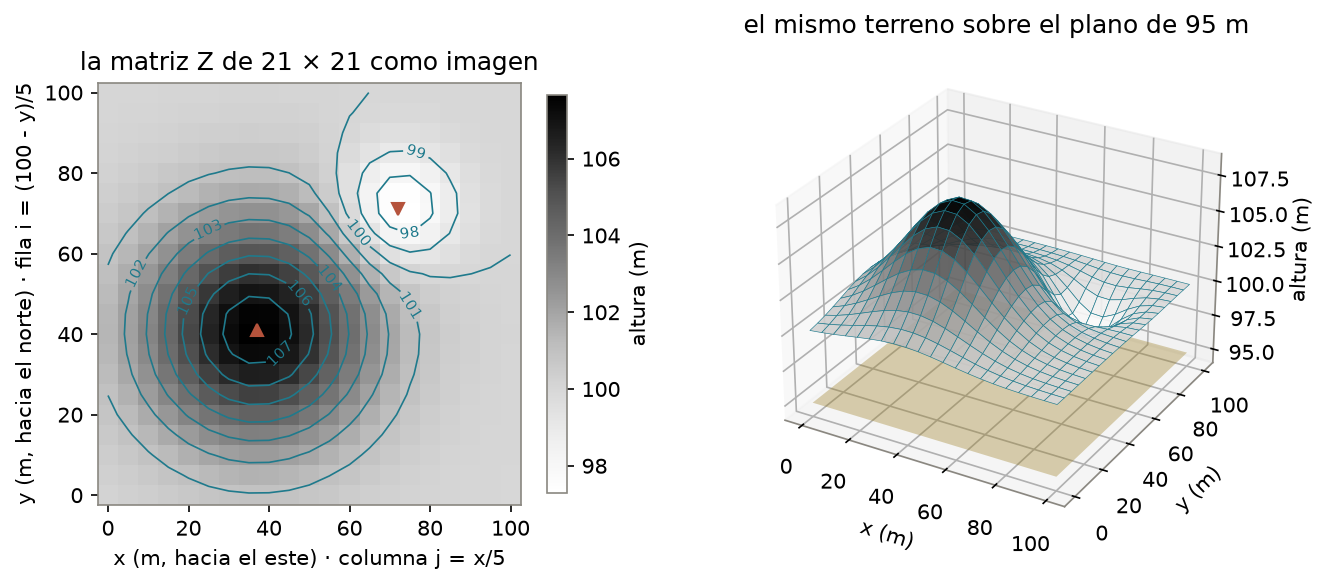
\includegraphics[width=\textwidth]{figuras/terreno-matriz/terreno_planilla.png}
\caption{El terreno de juguete. Izquierda: la matriz \(Z\) de \(21\times21\) pintada como una
foto en blanco y negro (más oscuro, más alto), con las líneas de igual altura cada \(1\) m; los
triángulos marcan el centro de la loma y el de la hondonada. Derecha: la misma matriz como
superficie, sobre el plano horizontal de \(95\) m de la aplicación. Generada con
\texttt{apunte/scripts/c3\_terreno\_matriz.py}.}
\label{fig:terreno-planilla}
\end{figure}

Las líneas de la figura~\ref{fig:terreno-planilla} unen puntos de igual altura; en los planos se
llaman \emph{curvas de nivel} y en \enquote{En profundidad} vemos cómo se trazan a partir de la
matriz. Donde las líneas se aprietan el terreno es empinado; donde se separan, es suave.

Mirar el terreno como matriz no es solo una manera de guardarlo. Las operaciones de matrices
tienen lectura directa. Sumar a \(Z\) una matriz constante es subir o bajar todo el terreno sin
cambiarle la forma. Multiplicar \(Z-100\) por \(2\) y volver a sumar \(100\) es exagerar el
relieve al doble sobre el llano. Restar dos matrices de alturas del mismo lugar, tomadas en dos
fechas, da cuánto se rellenó o se excavó en cada nodo. Invertir el orden de las filas es
espejar el terreno de norte a sur. Y transponer \(Z\) es reflejarlo respecto de la diagonal que
une la esquina noroeste con la sureste: cambia filas por columnas.

\subsection{Pendiente y orientación por diferencias}\label{sec:terreno-pendiente}

Imaginá que estás parado en un nodo de la ladera. ¿Cuánto se inclina el suelo y hacia dónde
correría el agua? Si tuviéramos la fórmula de la altura, la respuesta la darían las dos
derivadas parciales, cuánto sube el terreno por cada metro hacia el este y por cada metro hacia
el norte, puestas en una fila: el gradiente \(\nabla h=(\partial_xh\ \ \partial_yh)\), que el
capítulo~\ref{cap:derivada} estudia en detalle y que la sección~\ref{sec:gradiente-forma} ya
presentó como forma lineal. Pero en la matriz no hay fórmula: hay números en nodos separados
\(5\) m. Hacemos lo de la escalera de \enquote{La idea}: comparamos el vecino de adelante con el
de atrás y dividimos por lo que avanzamos entre los dos, \(2\Delta\). Esas cuentas se llaman
\emph{diferencias centradas}:
\[
  \partial_xh\approx\frac{z_{i,j+1}-z_{i,j-1}}{2\Delta},\qquad
  \partial_yh\approx\frac{z_{i-1,j}-z_{i+1,j}}{2\Delta}.
\]
En la segunda va primero la fila de arriba, \(i-1\), porque está al norte. Con el gradiente
aproximado salen dos números que interesan en el terreno. La \emph{pendiente} es cuánto se sube
por metro avanzado en la dirección más empinada, el largo \(\lVert\nabla h\rVert\); se da en
por ciento (metros que se suben cada \(100\) m) o como ángulo con la horizontal,
\(\arctan\lVert\nabla h\rVert\). La \emph{orientación} es hacia dónde mira la ladera, la
dirección en que baja más rápido, la del vector \(-\nabla h\) leído como flecha
\((-\partial_xh;\ -\partial_yh)\) (componente este, componente norte); la medimos como el
ángulo \(\mathrm{Az}\) que esa flecha forma con el norte, en sentido horario, como en la tabla
de notación del capítulo~0.

\begin{ejemplo}[Pendiente y orientación en un nodo]\label{ej:terreno-pendiente}
Tomamos el nodo de la fila \(10\) y la columna \(13\), en \(x=65\) m, \(y=50\) m, sobre el flanco
de la loma que mira a la hondonada. Su vecindario de \(3\times3\) en la matriz es
\[
  \begin{pmatrix}102{,}66&101{,}54&100{,}65\\103{,}41&\mathbf{102{,}33}&101{,}43\\103{,}84&102{,}74&101{,}82\end{pmatrix}\ \text{m}
\]
(fila de arriba, la del norte). Las diferencias centradas con \(\Delta=5\) m dan
\[
  \partial_xh\approx\frac{101{,}43-103{,}41}{10}=-0{,}198,\qquad
  \partial_yh\approx\frac{101{,}54-102{,}74}{10}=-0{,}120 .
\]
El terreno baja hacia el este y hacia el norte. La pendiente es
\(\sqrt{0{,}198^2+0{,}120^2}=0{,}2315\): \(23{,}15\) por ciento, o \(13{,}04^\circ\) con la
horizontal. La bajada apunta en la dirección \((0{,}198;\ 0{,}120)\), y su ángulo con el norte
es \(\arctan(0{,}198/0{,}120)=58{,}8^\circ\): la ladera mira al noreste, hacia la hondonada.

Como el terreno es de juguete, podemos comparar con la verdad. Derivando la fórmula de \(h\) en
\((65;\ 50)\) el gradiente exacto es \((-0{,}2027;\ -0{,}1186)\), con pendiente \(23{,}49\) por
ciento y orientación \(59{,}7^\circ\). Sin redondear las alturas a centímetros, las diferencias
centradas dan \((-0{,}1988;\ -0{,}1201)\) y \(23{,}22\) por ciento: el error en el gradiente es
de \(0{,}0043\). Si en lugar de los vecinos inmediatos usamos los que están a dos nodos
(paso efectivo de \(10\) m, la escalera de a cuatro escalones) el resultado empeora a
\((-0{,}1879;\ -0{,}1218)\), \(22{,}39\) por ciento y \(57{,}1^\circ\), con un error de
\(0{,}0152\): \(3{,}6\) veces más grande con el doble de paso. La
proposición~\ref{prop:terreno-centrada} de \enquote{En profundidad} explica por qué el error crece
como el cuadrado del paso, y por qué acá da \(3{,}6\) y no exactamente \(4\).
\end{ejemplo}

\begin{figure}[htbp]
\centering
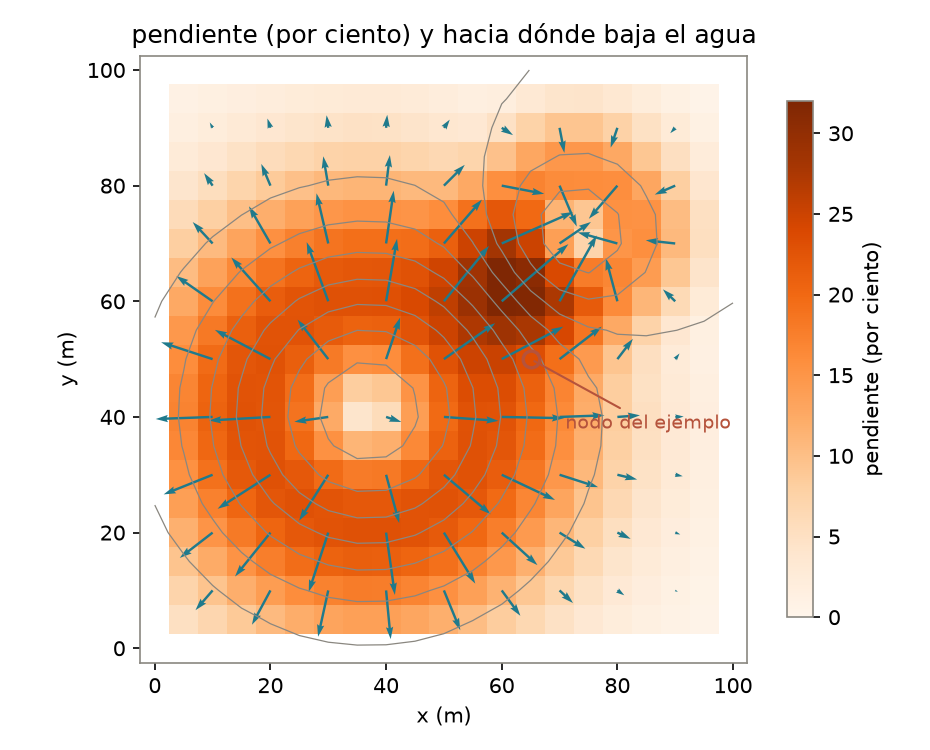
\includegraphics[width=.72\linewidth]{figuras/terreno-matriz/terreno_pendiente.png}
\caption{Pendiente del terreno de juguete calculada en cada nodo interior con diferencias
centradas (color, en por ciento) y la dirección de la bajada, \(-\nabla h\) (flechas, una de
cada dos nodos). El círculo marca el nodo del ejemplo~\ref{ej:terreno-pendiente}. En la cima de la
loma y en el fondo de la hondonada la pendiente se anula y la orientación no está definida.}
\label{fig:terreno-pendiente}
\end{figure}

Cerca de la cima de la loma la pendiente se anula, las flechas se achican y la orientación
deja de tener sentido: un terreno horizontal no mira hacia ningún lado. Es el mismo caso que el
gradiente nulo de un punto crítico (sección~\ref{sec:hessiana}).

\unidadInteractiva{10_jacobiano_primera_forma}{Jacobiano y primera forma fundamental}{Verificá: elegí la superficie «la loma r = (u, v, 2·exp(−(u²+v²)/8))» y dejá el punto en «u del punto» \(=2\), «v del punto» \(=1\). La tercera fila de \(J\) es el gradiente de la altura, \((\partial_uh\ \ \partial_vh)\); comprobá que da unos \((-0{,}535;\ -0{,}268)\). Calculá a mano la diferencia centrada con paso \(0{,}25\), \((h(2{,}25;\,1)-h(1{,}75;\,1))/0{,}5=(0{,}9374-1{,}2036)/0{,}5=-0{,}5324\), y compará. Después llevá el punto a la cima \((0,0)\) y mirá qué pasa con esa fila.}

\subsection{Volumen: una suma de prismas}\label{sec:terreno-volumen}

Supongamos que hay que bajar todo el terreno hasta un plano horizontal. ¿Cuánta tierra sale?
Entre el plano y la superficie queda un sólido, y su volumen es la integral doble de la altura
sobre el plano, \(\iint (h-z_0)\,dx\,dy\), donde \(z_0\) es la altura del plano. Con la matriz
no hay integral que hacer, pero sí una suma. Cada celda de la cuadrícula, el cuadrado de lado
\(\Delta\) que tiene cuatro nodos en las esquinas, es la base de un prisma; le damos como altura
el promedio de las alturas de sus cuatro esquinas sobre el plano. El volumen es la suma de los
prismas:
\[
  V\approx\Delta^2\sum_{\text{celdas}}\Bigl(\frac{z_{\mathrm{NO}}+z_{\mathrm{NE}}+z_{\mathrm{SE}}+z_{\mathrm{SO}}}{4}-z_0\Bigr).
\]
Cada nodo interior es esquina de cuatro celdas y cada nodo del borde, de dos (o de una, si es
una esquina del cuadrado). Sumando celda por celda, cada nodo aparece con peso \(1\) en el
interior, \(\tfrac12\) en el borde y \(\tfrac14\) en las cuatro esquinas, por \(\Delta^2\). La
proposición~\ref{prop:terreno-prisma} muestra que esta suma es el volumen exacto de la superficie
que se obtiene completando cada celda con la mezcla de sus cuatro esquinas que vemos en la
sección~\ref{sec:terreno-remuestreo}.

\begin{ejemplo}[Volumen de una celda y de todo el terreno]\label{ej:terreno-volumen}
Sobre el plano \(z_0=95\) m, la celda entre las filas \(10\) y \(11\) y las columnas \(8\) y \(9\),
cerca de la cima, tiene esquinas \(106{,}88\) (noroeste), \(106{,}41\) (noreste), \(106{,}96\)
(sureste) y \(107{,}46\) m (suroeste). Su promedio es \(106{,}93\) m, \(11{,}93\) m sobre el plano, y
el prisma tiene \(25\cdot11{,}9275=298{,}19\) m\(^3\).

Sumando los \(20\cdot20=400\) prismas de la cuadrícula se obtienen \(66\,218{,}9\) m\(^3\): una
capa de \(6{,}622\) m de espesor medio sobre los \(10\,000\) m\(^2\). Como la loma y la hondonada son
exponenciales de cuadrados, la integral de la fórmula se puede hacer exacta (cada exponencial se
separa en un factor que depende de \(x\) y otro de \(y\), y cada uno se integra con la función
error, \(\operatorname{erf}\)) y da \(66\,242{,}4\) m\(^3\). La suma de prismas se queda corta por
\(23{,}5\) m\(^3\), menos de cuatro diezmilésimos del total.

Un error frecuente es tomar cada nodo como una columna de \(5\times5\) m y sumar las \(441\)
columnas: da \(71\,641\) m\(^3\), un \(8{,}15\) por ciento de más. Las columnas de los nodos del borde
se salen del cuadrado: es como medir un terreno de \(105\) por \(105\) m. Los pesos \(\tfrac12\) y
\(\tfrac14\) del borde y de las esquinas corrigen eso.
\end{ejemplo}

\subsection{Remuestrear: pasar las alturas a otra cuadrícula}\label{sec:terreno-remuestreo}

¿Qué altura le damos a un punto que no es nodo? La pregunta aparece cada vez que hay que
entregar el terreno en otra cuadrícula, más gruesa, más fina o corrida, y a esa operación se la
llama \emph{remuestreo}. Las dos respuestas de \enquote{La idea} tienen nombre. La primera,
copiar la altura del nodo más cercano, es el \emph{vecino más próximo}: es rápida y no inventa
valores, pero el resultado es una superficie en escalones, con saltos donde cambia el nodo más
cercano. La segunda mezcla los cuatro nodos de la celda que contiene al punto. Si ponemos
coordenadas locales \((s,t)\in[0,1]^2\) en la celda (\(s\) hacia el este y \(t\) hacia el norte, en
unidades de paso) y llamamos \(f_{00}\), \(f_{10}\), \(f_{01}\), \(f_{11}\) a las alturas de las
esquinas suroeste, sureste, noroeste y noreste,
\[
  f(s,t)=(1-s)(1-t)\,f_{00}+s(1-t)\,f_{10}+(1-s)\,t\,f_{01}+s\,t\,f_{11}.
\]
Cada esquina pesa más cuanto más cerca está el punto, los cuatro pesos suman \(1\) y en cada
esquina \(f\) devuelve la altura medida. Es lineal a lo largo de cada recta paralela a los
lados de la celda (de ahí el nombre, \emph{bilineal}) pero no es un plano: tiene un término en
\(st\) que la tuerce. Es la misma función que usamos en \enquote{En profundidad} para trazar las
curvas de nivel dentro de una celda.

Cuál se equivoca menos depende del terreno, y lo medimos en la aplicación que sigue.

\subsection{Aplicación: un terreno de juguete y el volumen de un desmonte}\label{sec:terreno-aplicacion}

Antes de construir sobre un terreno con lomas hay que dejarlo horizontal. Si la plataforma
queda por debajo del terreno, hay que sacar la tierra que sobra por encima de ella: eso se
llama \emph{desmonte}. Para presupuestar la obra hace falta saber cuánta tierra es (cuántos
metros cúbicos), dónde el terreno es más empinado (ahí la máquina trabaja peor y el agua de
lluvia corre más rápido) y qué se pierde si los datos se entregan en una cuadrícula más gruesa.
Las tres preguntas se contestan con la matriz de alturas.

Los datos son los del terreno de juguete: el cuadrado de \(100\) por \(100\) m, la matriz \(Z\) de
\(21\times21\) nodos cada \(5\) m y la plataforma a \(z_0=95\) m. El punto más bajo del terreno
está a \(97{,}30\) m, así que todo el cuadrado queda por encima del plano y todo es desmonte.

\paragraph{Cuánta tierra.} La suma de prismas del ejemplo~\ref{ej:terreno-volumen} da
\(66\,218{,}9\) m\(^3\) contra \(66\,242{,}4\) m\(^3\) de la integral exacta: con un paso de \(5\) m
la matriz alcanza para el presupuesto.

\paragraph{Dónde es empinado.} Las diferencias centradas en los \(19\times19\) nodos interiores
(figura~\ref{fig:terreno-pendiente}) dan una pendiente media de \(13{,}29\) por ciento y una máxima de
\(31{,}99\) por ciento en el nodo de la fila \(7\) y la columna \(12\) (\(x=60\) m, \(y=65\) m), en el
cuello entre la loma y la hondonada, donde las dos laderas se suman. Calculada con la fórmula
en los mismos nodos, la máxima es \(33{,}58\) por ciento: las diferencias centradas con paso de
\(5\) m suavizan un poco las zonas más empinadas.

\paragraph{Qué se pierde con otra cuadrícula.} Supongamos que nos piden el terreno en una
cuadrícula de \(10\) m cuyo primer nodo está en \((3;\ 3)\), corrida \(3\) m al este y \(3\) m al
norte respecto de la nuestra: \(10\times10\) nodos, de \(x=3\) a \(x=93\) m y lo mismo en \(y\).
Ningún nodo nuevo coincide con uno viejo, así que hay que remuestrear. Como tenemos la fórmula,
podemos medir el error de cada método nodo por nodo:

{\small
\begin{center}
\begin{tabular}{l rrr}
\toprule
& error RMS (m) & error máximo (m) & volumen sobre \(95\) m en \([3,93]^2\) (m\(^3\))\\
\midrule
vecino más próximo & \(0{,}319\) & \(0{,}959\) & \(55\,882\) \ (\(-0{,}77\) por ciento)\\
bilineal & \(0{,}039\) & \(0{,}197\) & \(56\,178\) \ (\(-0{,}25\) por ciento)\\
alturas de la fórmula & \(0\) & \(0\) & \(56\,213\) \ (\(-0{,}18\) por ciento)\\
integral exacta & & & \(56\,317\)\\
\bottomrule
\end{tabular}
\end{center}
}

El error RMS es la raíz del promedio de los errores al cuadrado, un error típico. El vecino más
próximo se equivoca ocho veces más que la bilineal, y la figura~\ref{fig:terreno-remuestreo} muestra
por qué: cada nodo nuevo toma la altura del nodo viejo que está \(2\) m al este y \(2\) m al norte,
de modo que todo el terreno queda corrido \(2{,}83\) m hacia el suroeste. Donde la pendiente es
fuerte, un corrimiento horizontal se convierte en un error de altura (con \(32\) por ciento de
pendiente, \(2{,}83\) m de corrimiento pueden ser hasta unos \(0{,}9\) m), y su signo depende de hacia dónde
mira la ladera: las manchas rojas y azules de la figura son las dos caras de la loma. La bilineal
no corre el terreno; solo lo aplana un poco dentro de cada celda, y se equivoca en centímetros.

La última fila separa los dos errores del volumen. Aun con las alturas exactas en los nodos
nuevos, la cuadrícula de \(10\) m se queda corta por \(104\) m\(^3\): es lo que pierde la suma de prismas
con celdas más grandes. La bilineal agrega solo \(35\) m\(^3\) más de error; el vecino, \(331\) m\(^3\). Y
la pendiente máxima, calculada con diferencias centradas sobre la cuadrícula de \(10\) m remuestreada
con la bilineal, baja a \(26{,}70\) por ciento: con el doble de paso la ladera más empinada se ve
más suave de lo que es.

\begin{figure}[htbp]
\centering
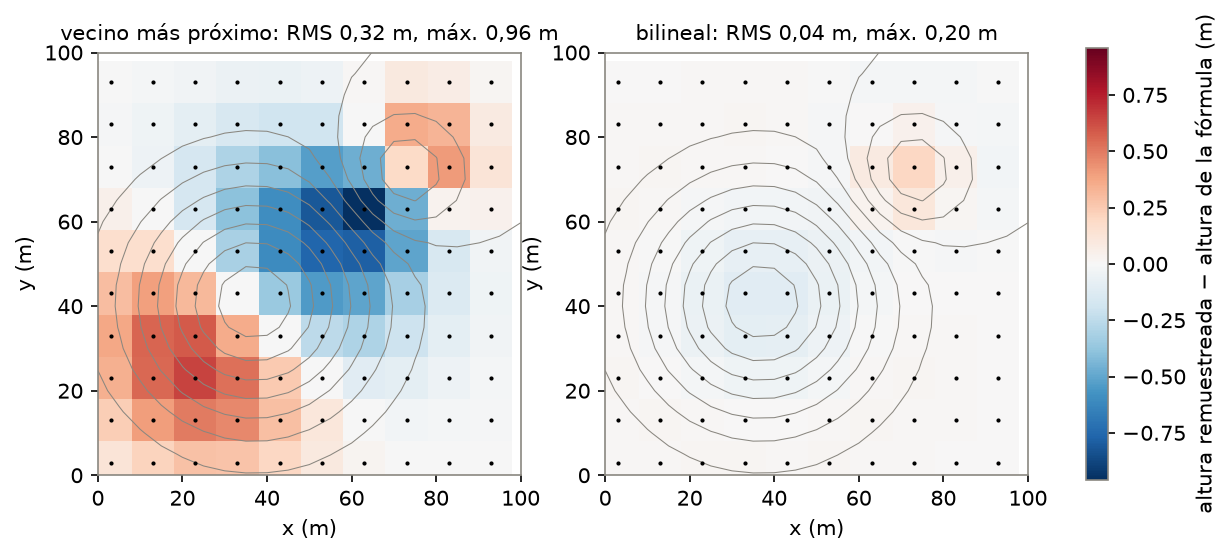
\includegraphics[width=\textwidth]{figuras/terreno-matriz/terreno_remuestreo.png}
\caption{Error de remuestrear el terreno de juguete a una cuadrícula de \(10\) m con origen en
\((3;\ 3)\) (puntos negros): altura remuestreada menos altura de la fórmula, con la misma escala de
color en los dos paneles. Izquierda, vecino más próximo; derecha, bilineal. En gris, las líneas de
igual altura cada \(1\) m.}
\label{fig:terreno-remuestreo}
\end{figure}

\begin{atencion}[Remuestrear no agrega información]
Pasar a una cuadrícula más gruesa pierde detalle que no se recupera: si después se vuelve a la
de \(5\) m, las alturas nuevas son mezclas de las de \(10\) m. Y el vecino más próximo, aunque no
invente valores, corre el terreno hasta medio paso: para alturas conviene la bilineal, y el
vecino solo cuando los valores son categorías (tipo de suelo, uso del terreno) que no se pueden
promediar.
\end{atencion}

\section{En profundidad}

\subsection{Por qué funcionan las cuentas de la cuadrícula}\label{sec:terreno-demostraciones}

Las dos cuentas de la sección anterior, la diferencia centrada y la suma de prismas, tienen una
justificación corta. La primera se apoya en el desarrollo de Taylor de una función de una
variable; la segunda, en integrar un polinomio en un cuadrado.

\begin{proposicion}[Error de la diferencia centrada]\label{prop:terreno-centrada}
Sea \(f\) una función con derivada tercera continua en \([x-k,\,x+k]\) y sea \(M\) un número mayor o igual
que \(\lvert f'''\rvert\) en todo ese intervalo. Entonces
\[
  \Bigl\lvert\frac{f(x+k)-f(x-k)}{2k}-f'(x)\Bigr\rvert\le\frac{M}{6}\,k^2 .
\]
\end{proposicion}

\begin{demostracion}
Por el desarrollo de Taylor con resto de Lagrange hasta el orden tres, existen \(\xi_+\in(x,x+k)\)
y \(\xi_-\in(x-k,x)\) tales que
\[
  f(x+k)=f(x)+f'(x)\,k+\tfrac12f''(x)\,k^2+\tfrac16f'''(\xi_+)\,k^3,\qquad
  f(x-k)=f(x)-f'(x)\,k+\tfrac12f''(x)\,k^2-\tfrac16f'''(\xi_-)\,k^3 .
\]
Restando, los términos en \(f(x)\) y en \(f''(x)\) se cancelan:
\(f(x+k)-f(x-k)=2f'(x)\,k+\tfrac16\bigl(f'''(\xi_+)+f'''(\xi_-)\bigr)k^3\). Dividiendo por \(2k\),
\[
  \frac{f(x+k)-f(x-k)}{2k}-f'(x)=\frac{f'''(\xi_+)+f'''(\xi_-)}{12}\,k^2 ,
\]
y el valor absoluto del numerador es a lo sumo \(2M\), lo que da la desigualdad.
\end{demostracion}

Para la derivada parcial \(\partial_xh\) se aplica a \(f(x)=h(x,y_i)\) con \(y\) fijo, y lo mismo
para \(\partial_yh\). La diferencia de un solo lado, \((f(x+k)-f(x))/k\), tiene en cambio un error
\(\tfrac12f''(x)\,k\) más términos de orden \(k^2\): es de primer orden, y por eso la tercera cuenta
de la escalera era la que menos se equivocaba. La desigualdad dice que el error es a lo sumo
proporcional a \(k^2\), y la fórmula de la demostración dice más: cuando \(k\) es chico, \(\xi_\pm\)
están cerca de \(x\) y el error se parece a \(\tfrac16f'''(x)\,k^2\), de modo que duplicar el paso
lo multiplica por casi \(4\). En el ejemplo~\ref{ej:terreno-pendiente} la razón fue \(3{,}6\): con
\(k=10\) m sobre una loma cuyo ancho característico es de unos \(20\) m, \(f'''\) ya cambia bastante
entre \(x\) y \(x\pm k\), y la aproximación \(f'''(\xi_\pm)\approx f'''(x)\) es gruesa.

\begin{proposicion}[La suma de prismas integra la bilineal]\label{prop:terreno-prisma}
Si \(f\) es la interpolación bilineal de los valores \(f_{00}\), \(f_{10}\), \(f_{01}\), \(f_{11}\) en
las esquinas de una celda cuadrada de lado \(\Delta\), entonces
\[
  \iint_{\text{celda}}f\,dA=\Delta^2\,\frac{f_{00}+f_{10}+f_{01}+f_{11}}{4}.
\]
En consecuencia, la suma de prismas de la sección~\ref{sec:terreno-volumen} es la integral exacta de
la superficie que completa cada celda con su bilineal.
\end{proposicion}

\begin{demostracion}
Con las coordenadas locales \(s=(x-x_0)/\Delta\), \(t=(y-y_0)/\Delta\), donde \((x_0,y_0)\) es la
esquina suroeste, se tiene \(dA=\Delta^2\,ds\,dt\). Desarrollando los productos de la fórmula de
la bilineal, \(f(s,t)=a+b\,s+c\,t+d\,st\) con
\[
  a=f_{00},\quad b=f_{10}-f_{00},\quad c=f_{01}-f_{00},\quad d=f_{00}-f_{10}-f_{01}+f_{11}.
\]
Como \(\int_0^1\!\int_0^1 ds\,dt=1\), \(\int_0^1\!\int_0^1 s\,ds\,dt=\int_0^1\!\int_0^1 t\,ds\,dt=\tfrac12\) y
\(\int_0^1\!\int_0^1 st\,ds\,dt=\tfrac14\),
\[
  \iint_{\text{celda}}f\,dA=\Delta^2\Bigl(a+\frac b2+\frac c2+\frac d4\Bigr).
\]
Reemplazando \(a\), \(b\), \(c\) y \(d\), el paréntesis vale
\(f_{00}\bigl(1-\tfrac12-\tfrac12+\tfrac14\bigr)+f_{10}\bigl(\tfrac12-\tfrac14\bigr)+f_{01}\bigl(\tfrac12-\tfrac14\bigr)+\tfrac14f_{11}
=\tfrac14\bigl(f_{00}+f_{10}+f_{01}+f_{11}\bigr)\). La segunda afirmación sale de sumar sobre las
celdas, porque la superficie bilineal por celdas es continua y la integral sobre el cuadrado es
la suma de las integrales sobre las celdas.
\end{demostracion}

Hecho geométrico: el prisma con la altura promedio de las cuatro esquinas tiene el mismo volumen
que el sólido de tapa torcida que forma la bilineal; lo que la tapa sube en un par de esquinas
opuestas lo baja en el otro, y el término en \(st\), que la tuerce, aporta lo mismo que si fuera
plano. Por eso el error de la suma de prismas no está en la suma: está en haber reemplazado el
terreno por la bilineal, y ese reemplazo mejora cuando la cuadrícula se afina. En el terreno de
juguete, con paso de \(5\) m el error fue de \(23{,}5\) m\(^3\) sobre \(66\,242\) m\(^3\), y con paso de
\(10\) m (y alturas exactas en los nodos) de \(104\) m\(^3\) sobre \(56\,317\) m\(^3\), en un cuadrado algo
menor. La celda de las curvas de nivel de más abajo da una comprobación: allí
\(f(s,t)=1496+8s+2t+2st\), su integral en la celda es \(1496+4+1+\tfrac12=1501{,}5\), y el promedio de
\(1496\), \(1504\), \(1508\) y \(1498\) es \(1501{,}5\).

\subsection{La SVD de un terreno real: del modelo digital de elevación a las curvas de nivel}\label{sec:svd-dem}
Un modelo digital de elevación es una
matriz: cada celda es una altura. El recorte de \(512\times512\) celdas del Copernicus DEM
GLO-30 sobre la Precordillera de Mendoza (\file{datos/dem\_copernicus/}, latitud
\(-32{,}284\) a \(-32{,}142\), longitud \(-69{,}000\) a \(-68{,}858\), una celda
\(\approx30\) m) tiene alturas entre \(1014\) y \(2989\) m, con desvío \(406\) m. Como
matriz tiene \(512\) valores singulares, ordenados de mayor a menor, y quedarse con los
\(k\) primeros términos \(\sigma_iu_iv_i^T\) es la mejor aproximación de rango \(k\): el
mismo problema 4 de la sección~\ref{cap:cuatro-problemas}, en grande. Los valores salieron
de \file{svd\_dem\_proto.py}, corrido fuera del navegador (la SVD completa tarda
\(0{,}06\) s en un M1):

{\small
\begin{center}
\begin{tabular}{l rrrrrrr}
\toprule
\(k\) (términos) & 1 & 2 & 5 & 10 & 20 & 50 & 100\\
\midrule
error RMS (m) & 103 & 66 & 31 & 17 & 9{,}8 & 4{,}4 & 2{,}0\\
\bottomrule
\end{tabular}
\end{center}
}

Hecho geométrico: una matriz constante es de rango \(1\), y la altura media del recorte
(unos \(1600\) m) es la \enquote{meseta} sobre la que está apoyado el relieve. Por eso
\(\sigma_1\) domina y la energía acumulada \(\sum_{i\le k}\sigma_i^2/\sum\sigma_i^2\) ya
da \(99{,}6\)\,\% con \(k=1\): esa cifra engaña, mide la meseta y no el relieve. El RMS
del error, o restar la media antes de descomponer (lo mismo que centrar la nube de puntos
en el problema 4), muestra lo que importa: el relieve \enquote{aparece} alrededor de \(k=20\)
(error de \(9{,}8\) m sobre un terreno de casi \(2000\) m de desnivel, la diferencia de altura entre su punto más bajo y el más alto) y con \(100\)
términos de \(512\) el error es de \(2\) m. La unidad \texttt{09\_cambio\_de\_base\_svd}
(apéndice~\ref{ap:notebooks}) carga ese mismo recorte y deja mover \(k\) en vivo.

\unidadInteractiva{09_cambio_de_base_svd}{Cambio de base y SVD}{Explorá: en la parte del recorte de la Precordillera, mové «k (valores singulares que conservamos)» de \(1\) a \(50\) y mirá cuándo aparecen los cerros chicos del centro. Comprobá que con \(k=20\) el error RMS de la submuestra de \(128\times128\) es de unos \(9{,}8\) m, el de la tabla de arriba.}

% --- 09-svd-nivel3 (redactado 2026-10-18) ---

Este complemento extiende la lectura de la SVD al terreno con el mismo recorte de Copernicus que usa la unidad \texttt{09\_cambio\_de\_base\_svd}. Todos los números salen de \texttt{np.linalg.svd} sobre la matriz de \(512\times512\) (\file{apunte/figuras/svd/gen\_dem\_curvas\_nivel.py}).

\subsubsection{El modelo digital de elevación como matriz y como función}

Como vimos en la sección~\ref{sec:terreno-planilla}, un modelo digital de elevación es una tabla
de alturas tomadas sobre una cuadrícula regular. En el recorte de la Precordillera, la fila \(i\) corresponde a una latitud (de norte
a sur, desde \(-32{,}142^\circ\) hasta \(-32{,}284^\circ\)), la columna \(j\) a una longitud
(de oeste a este, desde \(-69{,}000^\circ\) hasta \(-68{,}858^\circ\)) y la entrada
\(z_{ij}\) es la altura en metros. El paso de la cuadrícula es de un segundo de arco en las dos
direcciones; sobre el elipsoide de referencia del capítulo~\ref{cap:elipsoide}, a la latitud media del recorte, un segundo de latitud
mide \(30{,}80\) m y un segundo de longitud \(26{,}19\) m. El recorte cubre
\(15{,}8\) km de norte a sur por \(13{,}4\) km de este a oeste, con alturas entre
\(1014\) y \(2989\) m, media \(1626\) m y desvío \(406\) m.

La misma tabla admite dos lecturas, y las dos nos sirven.

\begin{itemize}
  \item \textbf{Como matriz} \(Z\in\R^{512\times512}\). Cada fila es un perfil
  oeste--este del terreno a latitud fija; cada columna, un perfil norte--sur a longitud fija.
  Sumar matrices es sumar relieves; multiplicar por un número es exagerar o aplanar el
  relieve.
  \item \textbf{Como muestra de una función} \(z=f(x,y)\) definida en todo el rectángulo,
  de la que solo conocemos los valores en los nodos: \(z_{ij}=f(x_j,y_i)\). La cuadrícula es
  la regla con que leemos el terreno, en el sentido de la
  sección~\ref{sec:puntos-formas-grillas}: los números \((i,j)\) no son metros sino marcas
  de dos mazos de rectas, uno de meridianos y otro de paralelos.
\end{itemize}

La primera lectura es la que permite descomponer; la segunda, la que permite hablar de
gradiente, plano tangente y curvas de nivel. Lo que sigue va y viene entre las dos.

\subsubsection{La SVD del terreno: una suma de relieves separables}\label{sec:svd-dem-separables}

Como cualquier matriz, \(Z\) se escribe
\[
  Z=U\Sigma V^T=\sum_{i=1}^{512}\sigma_i\,u_i\,v_i^T ,
  \qquad \sigma_1\ge\sigma_2\ge\dots\ge\sigma_{512}\ge0 .
\]
Cada término \(\sigma_iu_iv_i^T\) es una matriz de rango uno, y una matriz de rango uno
tiene una forma muy particular: su entrada \((r,c)\) es \(\sigma_i\,(u_i)_r\,(v_i)_c\), el
producto de un número que depende solo de la fila por otro que depende solo de la columna.

\paragraph{Hecho geométrico: el relieve separable.} Un término de rango uno es un relieve
que se obtiene tomando un perfil norte--sur \(u_i\) y un perfil oeste--este \(v_i\) y
multiplicándolos punto a punto. Todos sus perfiles oeste--este tienen la misma forma
\(v_i\), escalada por el valor de \(u_i\) en esa latitud; todos sus perfiles norte--sur tienen
la forma \(u_i\). Escalera: en \(\R\), un número es un relieve de una sola celda; en
\(\R^2\), una matriz de rango uno es un terreno \enquote{tejido} con un solo hilo en cada
dirección; la SVD dice que cualquier terreno es una suma de esos tejidos, ordenados por
importancia. Los vectores \(u_i\) y \(v_i\) son unitarios y adimensionales, de modo que
\(\sigma_i\) lleva las unidades de la altura: es la \enquote{amplitud} del tejido \(i\).

Los cinco primeros valores singulares del recorte son
\[
  \sigma_1=856\,621\ \text{m},\quad
  \sigma_2=40\,405\ \text{m},\quad
  \sigma_3=22\,048\ \text{m},\quad
  \sigma_4=18\,308\ \text{m},\quad
  \sigma_5=8\,784\ \text{m},
\]
y siguen bajando: \(\sigma_{20}=1467\) m, \(\sigma_{50}=453\) m, \(\sigma_{100}=170\) m. El
primero es más de veinte veces el segundo. La razón está en la meseta del remate: si \(Z\) fuera
constante e igual a la media \(\bar z\), sería \(\bar z\) por la matriz de unos, de rango uno,
con \(\sigma_1=\bar z\cdot512\) y \(u_1=v_1=\tfrac1{\sqrt{512}}(1,\dots,1)\). En el
recorte real \(\sigma_1/(\bar z\cdot512)=1{,}029\), y las entradas de \(u_1\) van de
\(0{,}0406\) a \(0{,}0461\), alrededor de \(1/\sqrt{512}=0{,}0442\): el perfil norte--sur del
primer término es casi plano. Las de \(v_1\) van de \(0{,}0302\) a \(0{,}0678\): el perfil
oeste--este baja a menos de la mitad, como el terreno, cuya altura media por columna pasa de
\(2563\) m en el borde oeste a \(1141\) m en el borde este. El primer término es entonces una
meseta inclinada hacia el este, con alturas entre \(1048\) y \(2677\) m.

\paragraph{Cuánto explica cada término.} Truncar la suma en \(k\) términos da
\(Z_k=\sum_{i\le k}\sigma_iu_iv_i^T\), la mejor aproximación de rango \(k\) de \(Z\): ninguna
otra matriz de rango \(k\) queda más cerca en la norma de Frobenius, la raíz de la suma de los
cuadrados de las entradas (es el problema 4 de la sección~\ref{cap:cuatro-problemas}). Como
las columnas de \(U\) y de \(V\) son ortonormales, los términos son perpendiculares entre sí
como matrices, y Pitágoras da
\[
  \|Z\|_F^2=\sum_{i}\sigma_i^2,\qquad
  \|Z-Z_k\|_F^2=\sum_{i>k}\sigma_i^2,\qquad
  \mathrm{RMS}_k=\sqrt{\frac{1}{512^2}\sum_{i>k}\sigma_i^2}\ .
\]
El error medio cuadrático en metros se lee directamente de los valores singulares que
descartamos, sin reconstruir nada. Comprobación con una matriz de juguete:
\(Z=\begin{pmatrix}12&11\\11&12\end{pmatrix}\) m, simétrica, con autovalores \(23\) y \(1\)
y autovectores \((1,1)\) y \((1,-1)\); sus valores singulares son \(23\) y \(1\), y
\(Z_1=23\cdot\tfrac12\begin{pmatrix}1&1\\1&1\end{pmatrix}\) es la meseta de \(11{,}5\) m. El
error \(Z-Z_1\) vale \(\pm0{,}5\) m en las cuatro celdas, su RMS es \(0{,}5\) m, y la fórmula
da \(\sqrt{1^2/4}=0{,}5\) m.

Para el recorte, con \(\|Z\|_F=858\,240\) m:

{\small
\begin{center}
\begin{tabular}{l rrrr}
\toprule
\(k\) & 1 & 5 & 10 & 20\\
\midrule
energía \(\sum_{i\le k}\sigma_i^2/\sum_i\sigma_i^2\) & \(99{,}62\)\,\% & \(99{,}967\)\,\% & \(99{,}990\)\,\% & \(99{,}997\)\,\%\\
error relativo \(\|Z-Z_k\|_F/\|Z\|_F\) & \(6{,}14\)\,\% & \(1{,}82\)\,\% & \(1{,}01\)\,\% & \(0{,}59\)\,\%\\
error RMS (m) & \(102{,}9\) & \(30{,}6\) & \(16{,}9\) & \(9{,}8\)\\
error máximo en una celda (m) & \(641\) & \(236\) & \(126\) & \(75\)\\
\bottomrule
\end{tabular}
\end{center}
}

Los RMS coinciden con los de la tabla del remate y con los que imprime la unidad
\texttt{09} con el repositorio clonado; en el navegador la unidad usa la submuestra de
\(128\times128\) (una celda de cada cuatro) y da \(103{,}5\), \(30{,}8\), \(17{,}0\) y
\(9{,}8\) m para los mismos \(k\). La primera fila muestra otra vez que la energía engaña: con
un solo término ya pasa del \(99{,}6\)\,\%, y sin embargo ese término se equivoca en \(103\) m
de RMS y en \(641\) m en la peor celda. Restando la media antes de descomponer, el primer
término deja de pagar la meseta y el RMS de \(k=1\) baja a \(85{,}4\) m; desde \(k\approx20\)
las dos versiones dan lo mismo. Para dibujar curvas de nivel la fila que importa es la del
RMS, porque se mide en las mismas unidades que la equidistancia.

\subsubsection{Curvas de nivel en una cuadrícula}\label{sec:svd-dem-curvas}

\paragraph{Definición.} La curva de nivel \(c\) de \(z=f(x,y)\) es el conjunto de los puntos
del plano donde \(f(x,y)=c\): la huella, proyectada sobre el plano horizontal, del corte del
terreno con el plano \(z=c\). En un plano topográfico se dibujan las curvas de una familia
equiespaciada, \(c=c_0+n\,e\), donde \(e\) es la \emph{equidistancia}; cada quinta curva es
maestra y lleva rotulada su altura.

\paragraph{Hecho geométrico: la curva de nivel es la recta de nivel cero del plano
tangente.} Cerca de un punto \(p\), el terreno se parece a su plano tangente,
\(f(p+h)\approx f(p)+df_p(h)\), donde \(df_p\) es la forma lineal que toma un desplazamiento
horizontal \(h\) y devuelve cuánto sube el terreno. Sus rectas de nivel son un mazo de
paralelas equiespaciadas, una regla graduada tirada sobre el plano
(sección~\ref{sec:puntos-formas-grillas}). Moverse a lo largo de la curva de nivel es moverse
sin subir ni bajar, es decir, en una dirección \(h\) con \(df_p(h)=0\): la tangente a la curva
de nivel es la recta de nivel cero de la forma \(df_p\), el núcleo de esa forma. Esta
afirmación no usa ninguna métrica. La que sí la usa es la otra, \enquote{el gradiente es perpendicular
a la curva de nivel}: para hablar de la dirección de máxima pendiente hay que convertir la
forma en un vector con el producto interno, y en la cuadrícula del recorte ese producto interno no es
el de los índices (secciones~\ref{sec:puntos-formas-grillas} y~\ref{cap:curvatura}). La
escalera: en \(\R\), la \enquote{curva} de nivel de \(z=f(x)\) es un punto aislado donde
\(f(x)=c\); en \(\R^2\), una curva; en \(\R^3\), las superficies de nivel de una función de
tres variables, como las superficies de igual temperatura o de igual potencial.

\paragraph{Una celda a mano.} En la cuadrícula solo tenemos alturas en los nodos. Dentro de cada
celda, entre cuatro nodos vecinos, completamos \(f\) de la manera más simple que respete los
cuatro valores: lineal a lo largo de cada lado de la celda. Una curva de nivel cruza un lado
exactamente cuando sus dos extremos quedan uno por encima y otro por debajo de \(c\), y el
punto de cruce se obtiene por interpolación lineal, como una regla de tres. Tomemos una celda
con coordenadas locales \((s,t)\in[0,1]^2\) (\(s\) hacia el este, \(t\) hacia el norte, en
unidades de celda) y alturas
\[
  f(0,0)=1496,\quad f(1,0)=1504,\quad f(1,1)=1508,\quad f(0,1)=1498\ \text{m},
\]
y busquemos la curva de \(1500\) m. El lado sur va de \(1496\) a \(1504\): lo cruza en
\(s=\frac{1500-1496}{1504-1496}=0{,}5\). El lado norte va de \(1498\) a \(1508\): lo cruza en
\(s=\frac{1500-1498}{1508-1498}=0{,}2\). Los lados oeste (\(1496\), \(1498\)) y este
(\(1504\), \(1508\)) no tienen cambio de signo. El tramo de curva dentro de la celda es el
segmento de \((0{,}5;\ 0)\) a \((0{,}2;\ 1)\).

\begin{center}
\begin{tikzpicture}[scale=2.4]
  \fill[teallight!40] (0,0)--(0.5,0)--(0.2,1)--(0,1)--cycle;
  \draw[mainline] (0,0) rectangle (1,1);
  \draw[rust,line width=1.2pt] (0.5,0)--(0.2,1);
  \fill (0,0) circle (0.7pt) node[below left,font=\small] {\(1496\)};
  \fill (1,0) circle (0.7pt) node[below right,font=\small] {\(1504\)};
  \fill (1,1) circle (0.7pt) node[above right,font=\small] {\(1508\)};
  \fill (0,1) circle (0.7pt) node[above left,font=\small] {\(1498\)};
  \node[font=\small,text=rust] at (0.62,0.5) {\(1500\)};
  \node[font=\small,text=muted] at (0.12,0.5) {\(-\)};
  \node[font=\small,text=muted] at (0.85,0.5) {\(+\)};
  \node[font=\footnotesize,below] at (0.5,-0.02) {\(s=0{,}5\)};
  \node[font=\footnotesize,above] at (0.2,1.02) {\(s=0{,}2\)};
\end{tikzpicture}
\end{center}

Con cuatro nodos y dos estados para cada uno (por encima o por debajo de \(c\)) hay
\(2^4=16\) configuraciones, que se reducen a cuatro casos. Si los cuatro nodos están del mismo
lado, la curva no entra en la celda. Si uno solo difiere, la curva corta la esquina de ese
nodo con un segmento entre los dos lados que llegan a él. Si dos nodos vecinos están de un
lado y los otros dos del otro, como en la celda de recién, un segmento atraviesa la celda.
Y si los nodos de una diagonal están por encima y los de la otra por debajo, hay cuatro
cruces y dos maneras de unirlos de a pares; el caso se decide con el valor del centro de la
celda, el promedio de los cuatro nodos, que dice si las dos esquinas altas están conectadas
por un lomo o separadas por un collado. Recorrer la cuadrícula celda por celda aplicando estos
cuatro casos y empalmar los segmentos que comparten un punto de cruce es, en lo esencial, lo que
hace una rutina de curvas de nivel como \texttt{matplotlib.pyplot.contour}.

\paragraph{La misma celda, leída con el gradiente.} La función que vale lo que vale en los
cuatro nodos y es lineal a lo largo de cada recta paralela a los lados (la interpolación
bilineal) es
\(f(s,t)=1496+8s+2t+2st\) (se verifica en los cuatro vértices). En el centro de la celda,
\(\partial f/\partial s=8+2t=9\) y \(\partial f/\partial t=2+2s=3\) metros por celda: la
forma lineal \(df=(9\ \ 3)\), cuyo núcleo es la dirección \((-1,3)\). El segmento que
trazamos tiene dirección \((0{,}2-0{,}5;\ 1-0)=(-0{,}3;\ 1)\), proporcional a
\((-1;\ 3{,}33)\): casi la recta de nivel cero del plano tangente. No coinciden del todo
porque el término \(2st\) curva la curva de nivel dentro de la celda (es un arco de hipérbola
y el segmento es su cuerda); en el centro, la curva verdadera pasa por \(t=0{,}444\) cuando
\(s=0{,}35\) y el segmento por \(t=0{,}5\), una diferencia de \(0{,}06\) celdas, menos de
\(2\) m sobre el terreno.

Ahora la métrica. Pasada a metros, con \(26{,}19\) m por celda hacia el este y \(30{,}80\) m
hacia el norte, la forma es \(df=(9/26{,}19\ \ \ 3/30{,}80)=(0{,}344\ \ 0{,}097)\), sin
unidades (metros de subida por metro de avance), y la tangente a la curva de nivel, que es
la misma dirección física, se escribe \((-26{,}19;\ 92{,}40)\) m; el producto da \(-9+9=0\), como
debe ser, porque el núcleo de una forma no depende de cómo graduemos los ejes. La dirección de
máxima pendiente, en cambio, es \((0{,}344;\ 0{,}097)\) en metros, que forma con el este un
ángulo de \(15{,}8^\circ\); el \enquote{perpendicular} calculado con los índices, \((9,3)\) en celdas,
corresponde en metros a \((235{,}7;\ 92{,}4)\), a \(21{,}4^\circ\) del este. Los
\(5{,}6^\circ\) de diferencia son la métrica de la cuadrícula geográfica que se olvida.

\subsubsection{Curvas de nivel sobre \texorpdfstring{$Z_k$}{Zk}: filtrar el relieve con la SVD}\label{sec:svd-dem-filtro}

La rutina de curvas de nivel acepta cualquier matriz de alturas. Si en lugar de \(Z\) le damos
\(Z_k\), dibuja las curvas de un terreno simplificado que conserva los \(k\) tejidos de mayor
amplitud. La figura~\ref{fig:svd-dem-curvas} muestra el resultado con la misma equidistancia
de \(50\) m y maestras cada \(250\) m en los cuatro paneles.

\begin{figure}[htbp]
\centering
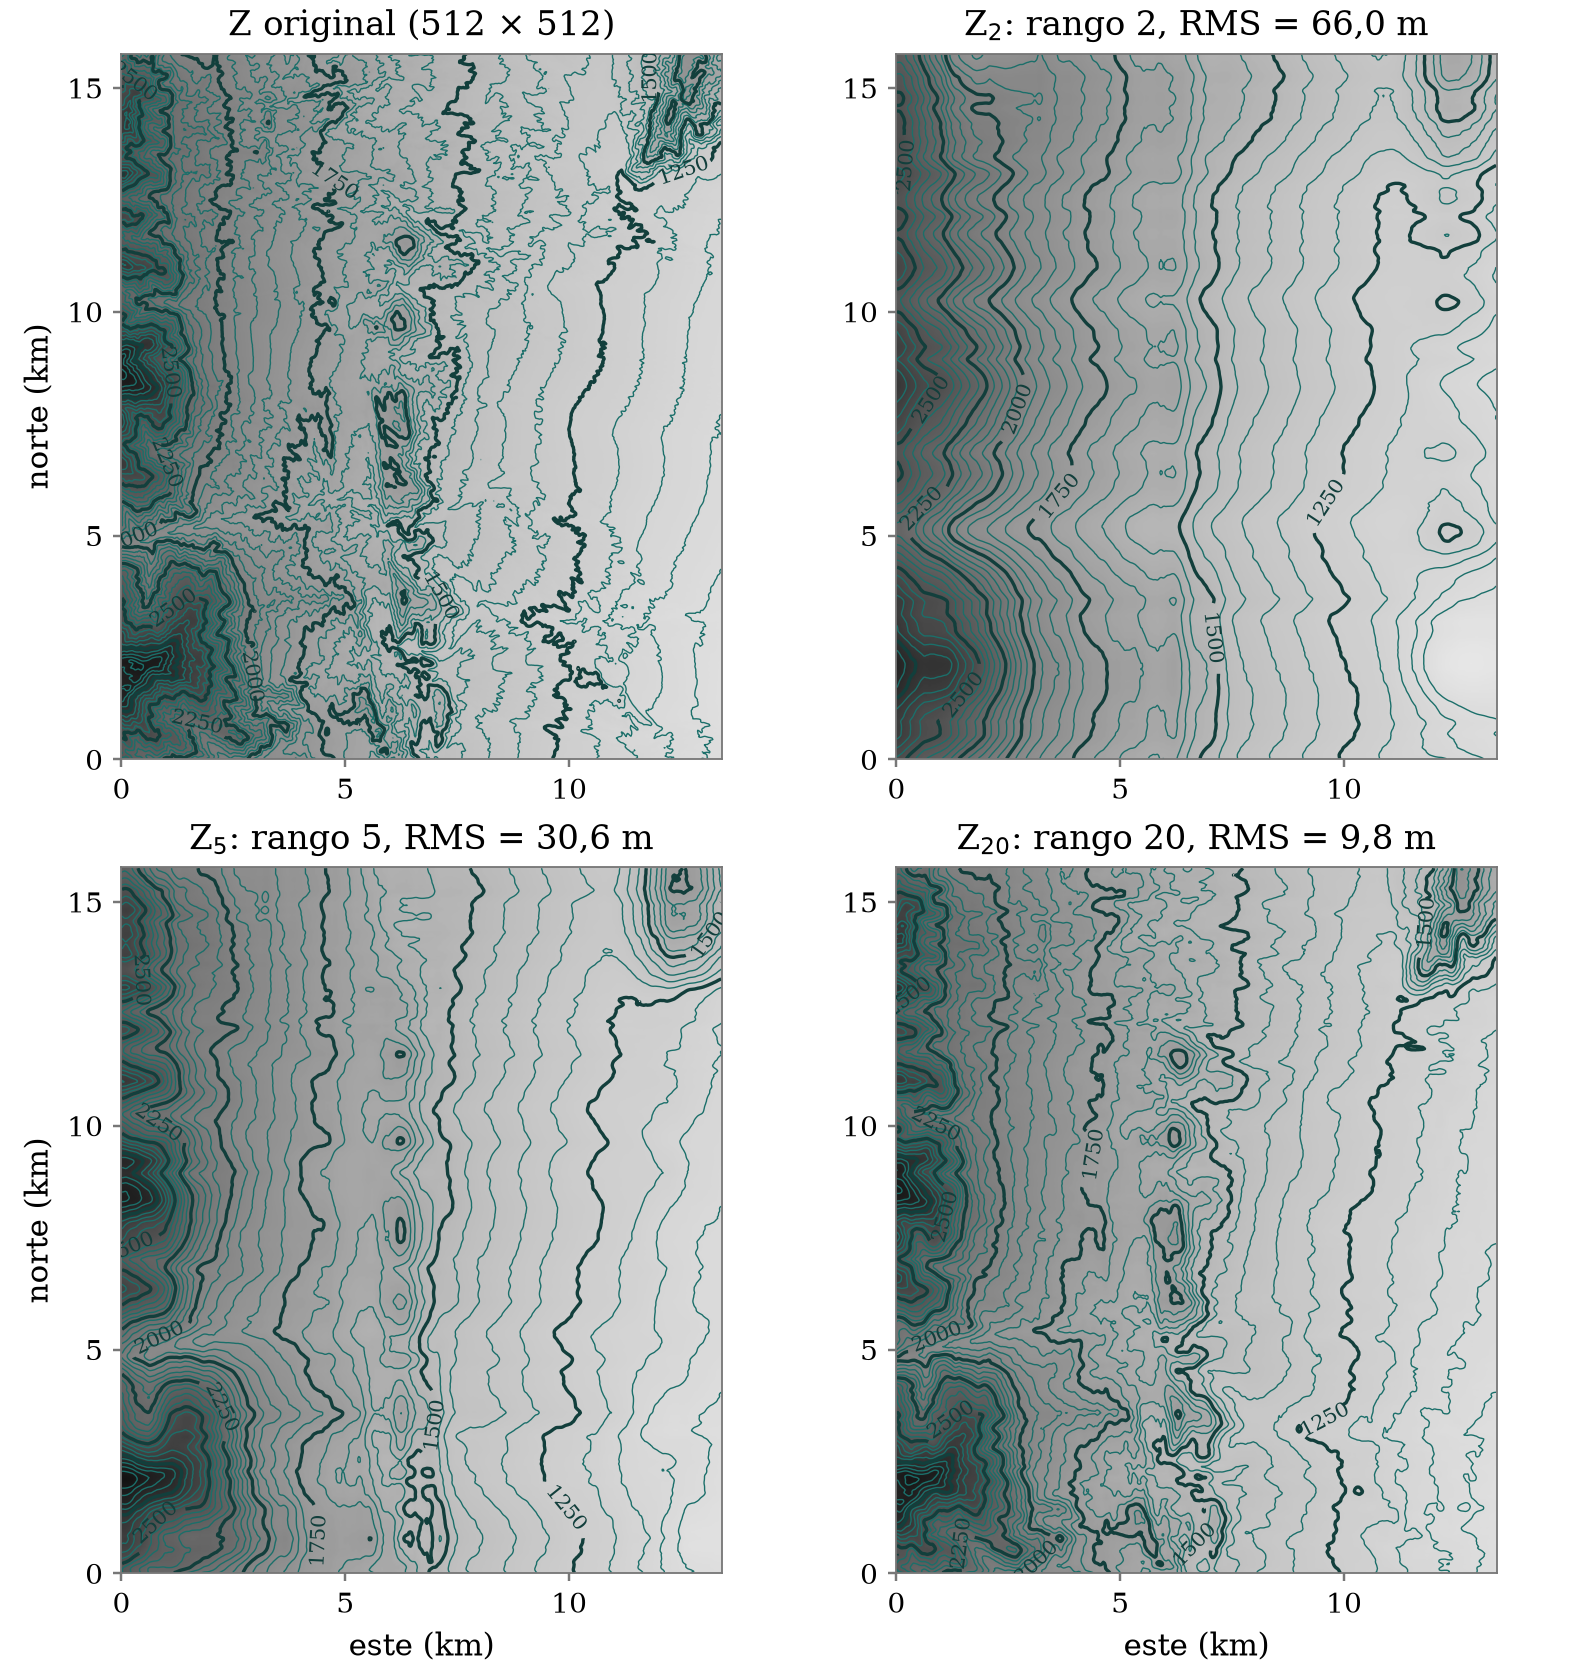
\includegraphics[width=\textwidth]{figuras/svd/dem_curvas_nivel.png}
\caption{Curvas de nivel del recorte de la Precordillera de Mendoza (Copernicus,
\(512\times512\) celdas de \(1''\)), equidistancia \(50\) m, maestras cada \(250\) m, trazadas
sobre la matriz original y sobre sus aproximaciones de rango \(2\), \(5\) y \(20\). El fondo gris
es la altura (más oscuro, más alto). Generada con
\texttt{apunte/figuras/svd/gen\_dem\_curvas\_nivel.py}. Datos: Copernicus DEM GLO-30, \enquote{\textcopyright{} DLR e.V. 2010-2014 and \textcopyright{} Airbus Defence and Space GmbH 2014-2018 provided under COPERNICUS by the European Union and ESA}.}
\label{fig:svd-dem-curvas}
\end{figure}

\paragraph{Lo que se ve.} Con \(k=2\) quedan las formas grandes: el cordón alto del oeste, el
descenso hacia el este y un par de lomas, todo con curvas de trazo largo y casi paralelas a
los meridianos. Es lo que cabe esperar de una suma de dos tejidos: cada uno tiene perfiles
norte--sur de una sola forma, de modo que las curvas tienden a alinearse con las columnas o con
las filas de la cuadrícula. Ese sesgo es propio del método, no del terreno: un cordón oblicuo a la
cuadrícula necesita muchos términos separables para quedar bien descripto. Con \(k=5\) aparecen
el cerro del ángulo noreste y los cerros del centro, todavía como manchas suaves. Con
\(k=20\) vuelve casi todo el dibujo: los cerros chicos alineados de norte a sur en el centro,
las entradas de las curvas en los cauces del oeste, los bordes quebrados de las maestras de
\(1500\) y \(1250\) m. Medido por el largo total de las curvas
de \(50\) m sobre el terreno, la matriz original tiene \(1174\) km de curvas repartidos en
\(307\) tramos; \(Z_{20}\) tiene \(923\) km en \(172\) tramos; \(Z_5\), \(716\) km en
\(119\); \(Z_2\), \(609\) km en \(83\). Cada término agregado agrega rugosidad, y una parte
de esa rugosidad es relieve y otra parte es ruido del propio modelo (es un modelo de superficie,
con vegetación y artefactos de medición, no de terreno desnudo).

\paragraph{Cuándo el filtro sirve y cuándo falsea.} Truncar la SVD es un filtro con una
ventaja clara: el error está controlado por números que conocemos antes de dibujar, los
\(\sigma_i\) descartados. Sirve cuando la escala del plano no puede mostrar el detalle: en
cartografía a escala chica, con equidistancia grande, las curvas de la matriz original salen
temblorosas y llenas de tramos cortos que el dibujante igual eliminaría a mano, y \(Z_k\) los
elimina con un criterio uniforme en toda la hoja. Falsea cuando lo que se busca es justamente
el detalle local: el talud de un camino, una cárcava, el borde de una terraza, el pie de un
cerro que define un límite. Un error RMS bajo es un promedio sobre \(262\,144\) celdas y no
garantiza nada en una celda en particular: con \(k=20\) el RMS es \(9{,}8\) m pero el error
llega a \(75\) m en la peor celda, aunque solo en el \(0{,}04\)\,\% de las celdas supera los
\(50\) m. Para un relevamiento de detalle, la matriz que manda es \(Z\), y conviene mirar
\(Z-Z_k\) como mapa para saber qué se está tirando.

\paragraph{Un criterio numérico para elegir \(k\).} Una curva de nivel está bien ubicada si
el error en altura es chico frente a la equidistancia: si el error vale la mitad de \(e\), la
curva puede confundirse con su vecina. Una regla práctica razonable es pedir
\[
  \mathrm{RMS}_k\le\frac{e}{5},
\]
y como \(\mathrm{RMS}_k\) se calcula solo con los \(\sigma_i\), el menor \(k\) que la cumple
se busca recorriendo la lista de valores singulares. En el recorte de la Precordillera:

{\small
\begin{center}
\begin{tabular}{r r r r r}
\toprule
equidistancia \(e\) & error admitido \(e/5\) & menor \(k\) & \(\mathrm{RMS}_k\) & error máximo\\
\midrule
\(100\) m & \(20\) m & \(9\) & \(18{,}7\) m & \(129\) m\\
\(50\) m & \(10\) m & \(20\) & \(9{,}8\) m & \(75\) m\\
\(25\) m & \(5\) m & \(44\) & \(4{,}95\) m & \(33\) m\\
\bottomrule
\end{tabular}
\end{center}
}

Para la equidistancia de la figura, \(50\) m, el criterio elige \(k=20\): veinte tejidos de
\(512\), y \(Z_{20}\) se guarda con \(20\cdot(512+512+1)=20\,500\) números en lugar de
\(262\,144\), menos del \(8\)\,\%. El error en altura se traduce en un corrimiento horizontal
de la curva que depende de la pendiente: donde el terreno sube \(\tan\theta\) metros por
metro, un error vertical \(\delta\) corre la curva unos \(\delta/\tan\theta\) metros. La
pendiente mediana del recorte es \(0{,}188\) (unos \(10{,}6^\circ\)), así que los \(9{,}8\) m
de \(Z_{20}\) mueven las curvas del orden de \(52\) m, dos celdas, en un terreno típico, y
bastante más en los llanos del este, donde la pendiente es menor. Es el mismo número visto de
otro modo: en escala \(1\!:\!50\,000\), \(52\) m son un milímetro del plano, el límite de lo
que se dibuja; en escala \(1\!:\!5000\) son un centímetro, y ahí \(k=20\) ya no alcanza.

\subsubsection{Conexiones con el resto del programa}\label{sec:svd-dem-conexiones}

\paragraph{El plano que mejor aproxima y la pseudoinversa.} El primer modelo de un terreno que se le
ocurre a un agrimensor no es \(Z_1\) sino un plano, \(z=a\,x+b\,y+c\), con \(x\) hacia el este
y \(y\) hacia el norte en metros. Ajustarlo es un sistema sobredeterminado de \(262\,144\)
ecuaciones con tres incógnitas, una por celda, \(a\,x_j+b\,y_i+c\approx z_{ij}\), que se
resuelve con la pseudoinversa de la sección~\ref{sec:pseudoinversa}: \((a,b,c)=A^{+}z\), con
\(A\) de \(262\,144\times3\) y columnas \(x\), \(y\) y unos. En el recorte da un plano que baja
\(97\) m por kilómetro hacia el este y sube \(4{,}4\) m por kilómetro hacia el norte
(pendiente de \(5{,}5^\circ\)), con un RMS de \(153{,}7\) m.

La comparación con la SVD es instructiva. El plano, escrito como matriz, es
\((b\,y_i+c)\cdot1+a\cdot x_j\): la suma de una matriz que solo depende de la fila y otra que
solo depende de la columna, de rango dos. Por lo tanto su error no puede ser menor que el de la
mejor aproximación de rango dos, y efectivamente \(153{,}7\ \text{m}>66{,}0\ \text{m}\). Lo
llamativo es que también pierde contra \(Z_1\), de rango uno, que da \(102{,}9\) m. La razón
es que el plano obliga a los perfiles a ser rectas, mientras que la SVD elige los perfiles que
mejor describen el terreno, y el perfil oeste--este real, que cae más de \(1400\) m en
\(13\) km de manera nada uniforme, no es una recta. Las dos aproximaciones son de mínimos cuadrados (minimizan la suma de los
cuadrados de las diferencias) con el mismo dibujo de la proyección ortogonal (caja \enquote{El dibujo único detrás de \(Ax\approx b\)}
de la sección~\ref{cap:cuatro-problemas}); lo que cambia es el subespacio sobre el que
proyectamos: planos en un caso, matrices de rango \(k\) en el otro.

\paragraph{La cuadrícula geográfica no es cuadrada.} Todo lo anterior trató a \(Z\) como una
tabla con celdas iguales, y la SVD lo hace sin preguntar: suma cuadrados de alturas celda por
celda. Pero las celdas de un segundo de arco no son cuadradas (\(30{,}80\) por \(26{,}19\) m
en este recorte) ni todas iguales: el ancho este--oeste es \(N\cos\varphi\) por un segundo
en radianes, con \(N\) la gran normal del elipsoide, y pasa de \(26{,}17\) m en el borde sur a
\(26{,}21\) m en el borde norte. En \(15\) km la variación es despreciable; en un modelo de elevación que cubre
varios grados de latitud no lo es, y una celda cerca del polo es una astilla. La cuadrícula
\((\lambda,\varphi)\) es una parametrización del elipsoide con primera forma fundamental
\(ds^2=N^2\cos^2\varphi\,d\lambda^2+M^2\,d\varphi^2\) (secciones~\ref{sec:metrica}
y~\ref{cap:elipsoide}). Para las curvas de nivel eso tiene dos consecuencias. El trazado
mismo no cambia, porque una curva de nivel es el núcleo de una forma y no necesita métrica.
Cambian todas las cuentas que miden: el largo de las curvas, las pendientes, la dirección de
máxima pendiente y el corrimiento horizontal de una curva por un error vertical, que en este
recorte hicimos convirtiendo celdas a metros con los dos factores de la métrica. Y si
quisiéramos que la propia SVD pesara cada celda por el área que representa, habría que
descomponer \(D_1^{1/2}\,Z\,D_2^{1/2}\), con \(D_1\) y \(D_2\) diagonales con los pesos de
filas y columnas: otra vez, la base privilegiada la elige la regla de medir.

\begin{resultado}[Lo que sabemos hacer con un modelo digital de elevación]
Leerlo como matriz \(Z\) y como muestra de una función \(z=f(x,y)\) en una cuadrícula geográfica.
Descomponerlo en tejidos separables \(\sigma_iu_iv_i^T\) y saber, solo con los \(\sigma_i\)
descartados, el error RMS en metros de la aproximación \(Z_k\). Trazar sus curvas de nivel
celda por celda por interpolación lineal, sabiendo que cada tramo aproxima la recta de nivel
cero del plano tangente. Y elegir \(k\) para que el error quede por debajo de una fracción de
la equidistancia (en la Precordillera, \(k=20\) para \(50\) m), sabiendo que el filtro sirve
para la forma grande y no para el detalle de un relevamiento.
\end{resultado}

\section{Ejercicios con solución}

\begin{ejercicio}\label{ex:terreno-pendiente}
Una planilla de alturas con paso de \(10\) m tiene, con la fila de arriba al norte,
\[
  \begin{pmatrix}104&106&109\\101&103&107\\99&100&104\end{pmatrix}\ \text{m}.
\]
Calculá con diferencias centradas el gradiente en el nodo central, la pendiente (en por ciento y
en grados) y la orientación de la bajada, medida desde el norte en sentido horario.
\end{ejercicio}
\solucion{\(\partial_xh\approx(107-101)/20=0{,}3\) y \(\partial_yh\approx(106-100)/20=0{,}3\) (la fila
de arriba, al norte, va con signo más). La pendiente es \(\sqrt{0{,}3^2+0{,}3^2}=0{,}424\): \(42{,}4\)
por ciento, o \(\arctan0{,}424=23{,}0^\circ\). El terreno sube hacia el noreste, así que baja en la
dirección \((-0{,}3;\ -0{,}3)\), hacia el suroeste: la orientación es \(225^\circ\).}

\begin{ejercicio}\label{ex:terreno-volumen}
Con la planilla del ejercicio~\ref{ex:terreno-pendiente}, calculá el volumen que queda por encima
del plano de \(99\) m con la suma de prismas de las cuatro celdas. Comprobá que da lo mismo
pesando cada nodo con \(1\), \(\tfrac12\) o \(\tfrac14\) según sea interior, de borde o de esquina, y
compará con lo que da tomar cada nodo como una columna de \(10\times10\) m.
\end{ejercicio}
\solucion{Los promedios de las cuatro celdas son \(103{,}5\), \(106{,}25\), \(100{,}75\) y \(103{,}5\) m,
es decir \(4{,}5\), \(7{,}25\), \(1{,}75\) y \(4{,}5\) m sobre el plano; sumados dan \(18\) m, y por
\(100\) m\(^2\) de cada celda, \(1800\) m\(^3\). Con pesos: esquinas
\(\tfrac14(5+10+0+5)=5\), bordes \(\tfrac12(7+2+8+1)=9\), centro \(4\); total \(18\) m, los mismos
\(1800\) m\(^3\). Las nueve columnas dan \(100\cdot42=4200\) m\(^3\), más del doble: con tan pocos nodos,
casi todos están en el borde y sus columnas se salen del cuadrado de \(20\times20\) m.}

\begin{ejercicio}\label{ex:terreno-bilineal}
En la celda de la sección~\ref{sec:svd-dem-curvas}, con alturas \(1496\) (suroeste), \(1504\)
(sureste), \(1508\) (noreste) y \(1498\) m (noroeste), calculá la altura bilineal en el punto
\((s,t)=(0{,}3;\ 0{,}6)\) y la que daría el vecino más próximo. ¿De qué lado de la curva de
\(1500\) m queda el punto según cada método? Verificá también que la integral de la bilineal en
la celda (de lado \(1\)) es el promedio de las cuatro esquinas.
\end{ejercicio}
\solucion{Con \(f(s,t)=1496+8s+2t+2st\), \(f(0{,}3;\ 0{,}6)=1496+2{,}4+1{,}2+0{,}36=1499{,}96\) m. La
esquina más cercana a \((0{,}3;\ 0{,}6)\) es la noroeste, \((0,1)\), y el vecino más próximo da
\(1498\) m. Los dos dejan el punto por debajo de \(1500\) m, pero la bilineal lo pone a \(4\) cm
de la curva y el vecino a \(2\) m: el vecino no ve que el punto está casi sobre ella. La integral
es \(1496+\tfrac82+\tfrac22+\tfrac24=1501{,}5\), igual a \((1496+1504+1508+1498)/4\), como dice la
proposición~\ref{prop:terreno-prisma}.}

\begin{ejercicio}\label{ex:terreno-operaciones}
A la matriz \(Q\) del ejercicio~\ref{ex:terreno-pendiente} se le aplican tres operaciones: (a) sumarle
\(10\) a todas las entradas; (b) exagerar el relieve al doble sobre el plano de \(99\) m, o sea
reemplazarla por \(99+2(Q-99)\); (c) invertir el orden de las filas. Para cada una, decí qué pasa
con la pendiente, con la orientación en el nodo central y con el volumen sobre el plano de
\(99\) m, sin rehacer todas las cuentas, y comprobalo.
\end{ejercicio}
\solucion{(a) Las diferencias no cambian: pendiente \(42{,}4\) por ciento y orientación
\(225^\circ\); el volumen crece en \(10\) m por los \(400\) m\(^2\), de \(1800\) a \(5800\) m\(^3\).
(b) Las diferencias se duplican: gradiente \((0{,}6;\ 0{,}6)\), pendiente \(84{,}9\) por ciento,
misma orientación \(225^\circ\); el volumen se duplica, \(3600\) m\(^3\). (c) Es espejar de norte a
sur: \(\partial_xh\) sigue en \(0{,}3\) y \(\partial_yh\) cambia de signo, \(-0{,}3\); la pendiente no
cambia y la bajada apunta a \((-0{,}3;\ 0{,}3)\), hacia el noroeste: \(315^\circ\), que es
\(180^\circ-225^\circ\) llevado a \([0^\circ,360^\circ)\). El volumen no cambia, \(1800\) m\(^3\): los prismas son
los mismos, en otro orden.}
